\section{Background}
% 
In this section, we will explain some of the main concepts used in this project. This section is needed to establish a common understanding behind these topics, so that unambiguous discussion can follow.

First we will briefly talk about the concept of currency and its exchange. Afterwards we will define what a cryptocurrency is and how it differs from a fiat currency. 
% 
\subsection{Fiat  currency}
% 
Currency, as the medium of exchange for goods and services, is the basis of trade. Since the history of humanity, we have always engaged in some sort of a trade. Whenever we needed a commodity we do not posses, we needed to get this commodity by trading it for something else. This exchange of commodities was referred to as barter trade. Barter trade, however was not always suitable, since it required the alignment of wants and was not very scalable for large transactions~\cite{Carroll2015CreatingExchange}. To overcome these limitations, money was invented. Money can be seen as opposition to barter trade. In the beginning, cattle, salt or precious metals were used as 'comodity money', later coins were invented. But money is not necessarily the same as `currency'.  Currency is more specific form of money. Currency, in traditional meaning is issued and controlled by the government\footnotemark.
% 
\footnotetext{\url{https://www.investopedia.com/terms/c/currency.asp}, accessed 22-03-2018}

Until 1971, every US dollar could be exchanged for its respective value in gold. This system is known as a ``representative currency'', since the entire currency is represented by the amount of gold the government posses. This is also called ``Gold standard'' and is currently rarely used. In opposition to representative currency stands the fiat currency. 

Fiat currency is a currency that is issued and controlled by the government and is declared a legal tender in respective country. However, unlike the representative currency, it is not backed by any physical commodity and its value is simply derived from the supply-demand relationship\footnotemark. Most of today's currencies, including US Dollars, Euros, Yens or Danish Crowns are fiat currencies.
% 
\footnotetext{\url{https://www.investopedia.com/terms/f/fiatmoney.asp}, accessed 22-03-2018}
% 
\subsection{Cryptocurrency}
% 
Merriam-Webster dictionary defines cryptocurrency as a \textit{``form of currency that only exists digitally, that usually has no central issuing or regulating authority, but instead uses a decentralised system to record transactions and manage the issuance of new units, and that relies on cryptography to prevent counterfeiting and fraudulent transactions''}\footnotemark.
% 
\footnotetext{\url{https://www.merriam-webster.com/dictionary/cryptocurrency}, accessed 27-03-2018}

Digital currency means that we can only access it in a digital world. This is opposed to fiat currencies, which have both physical representation of the currency (coins and notes) and digital representation (money in a bank). Technology of cryptography assures that the currency will only be used in the intended way. Fraud cases, such as producing additional fake currency, double spending, or unauthorised transfer need to be prevented. With the physical cash, measures can be taken to prevent tampering with the notes and coins, such as watermarks, special print or holograms. In the digital world, these measures need to be enforceable and verifiable by the computer.

There are numerous technical characteristics of cryptocurrencies. However, the most prominent ones, as listed by many research works~\cite{Lansky2018PossibleCryptocurrencies} are the following:
\begin{enumerate}[noitemsep]
    \item The system does not require a central authority, distributed entities achieve consensus on its state.
    \item The system keeps an overview of cryptocurrency units and their ownership.
    \item The system defines whether new cryptocurrency units can be created. If new cryptocurrency units can  be  created,  the  system  defines  the  circumstances  of  their  origin  and  how  to  determine  the ownership of these new units.
    \item Ownership of cryptocurrency units can be proved exclusively cryptographically.
    \item The system allows transactions to be performed in  which ownership of the cryptographic units is changed. A transaction statement can only be issued by an entity proving the current ownership of these units.
    \item If  two  different  instructions  for  changing  the  ownership  of the  same  cryptographic  units  are simultaneously entered, the system performs at most one of them.
\end{enumerate}

Public-key encryption and hashing are the two most used cryptographic concepts used in cryptocurrencies. In several cryptocurrencies, hashing is used to maintain a consensus over the network's state and public-key cryptography is used to prove the ownership of the cryptocurrency\footnotemark.
% 
\footnotetext{Not all currencies use the public-key cryptography. For example, Fawkescoin only uses hashing for both state consensus and currency ownership~\cite{Bonneau2014FawkescoinCryptography}}

\subsubsection{Motivation for cryptocurrencies}
Naturally, the cryptocurrency was not entering a blue ocean upon its inception. Today, all countries have a generally accepted currency, usually issued by central bank. This system, however, has certain limitations. The main drawback is virtually unlimited supply of the currency. A government can issue more money, as it deems necessary. As a consequence, the value of a fiat currency can therefore decrease drastically (e.g. the value of Zimbabwean dollar dropped by hundreds of percents in 2006~\cite{MichaelWines2006HowZimbabwe} or hyper-inflation case in Venezuela in 2018~\cite{ManuelRueda2018VenezuelasMoney}). Secondary, the government could use its ability to control the currency to influence anti-governmental organisations or groups by limiting their access to their funds. This can be a problem for whistle-blower organisations (such as WikiLeaks) or for freedom movements in repressive regimes.

Cryptocurrency overcomes these problems, since there is no central authority that could control the currency. Every user of the currency can participate in making the more secure by running specialised software on their computer. The issue of units of the currency is controlled by the system in a well-defined and expectable manner. The trust in the central bank is thus replaced by trust in the cryptocurrency. In the next section we will explore, how blockchain enables this decentralisation.
% 
\subsection{Blockchain}
% 
Since the inception of a digital currency Bitcoin (described in the following section) in 2009, blockchain has been part of the discussions about this novel approach to currency. Over the time, the perception shifted from seeing blockchain just as a part of cryptocurrency into seeing it as an separate, innovative, even disruptive technology. Some media mark \textit{blockchain} to be the word of the year 2017\footnotemark, while others comparable it to inception of the Web in 1990s \cite[p. 14]{Swan2015BlockchainEconomy}.
% 
\footnotetext{\url{https://www.theguardian.com/technology/2018/jan/30/blockchain-buzzword-hype-open-source-ledger-bitcoin}, accessed 28-03-2018}

From the perspective of cryptocurrency, blockchain is a public ledger, that contains all the transactions of the cryptocurrency to date \cite{Swan2015BlockchainEconomy}. It is distributed among all the computers participating in the consensus process. Since it contains all the past transactions (since the inception of the currency), data is never deleted from the blockchain. All changes happen only as amendments to the latest version of the blockchain.

A \textit{change} could be virtually any data. For example, it could be details of latest transactions (as is the case with Bitcoin) or newly deposited agreements (as in Quorum - enterprise level ledger \footnotemark ). This \textit{change} is called a \textit{block}. Blocks are the fundamental parts, that make up the blockchain. When a new blockchain is created, a first set of changes becomes the first block.
% 
\footnotetext{Quorum is a blockchain-based private storage for agreements. Its intended users are enterprises in the finance industry, who are trading financial derivatives and who need to reach an agreement, while maintaining acceptable level of privacy.
\begin{flushleft}
\url{http://fortune.com/2016/10/04/jp-morgan-chase-blockchain-ethereum-quorum/}, accessed 28-03-18
\url{https://www.jpmorgan.com/global/Quorum}, accessed 28-03-18
\end{flushleft}
}
% 
When more changes are made (for example, more transactions are processed), a new block is created. The creation of a new block involves computing a hash value of the previous block. This hash value is then included in the new block, together with the data comprising the change. By including the hash value of the old block in the new block, these two blocks are now linked. All the blocks in the blockchain are linked together in such fashion. Figure \ref{fig:blockch-basics} illustrates this principle. 
% 
\begin{figure}[h]
    \centering
    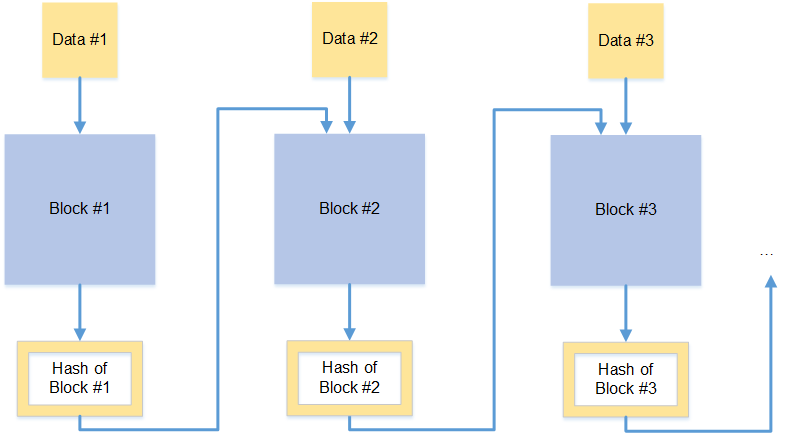
\includegraphics[width=.95\textwidth]{blockchain-basics}
    \caption{The basic architecture of a blockchain. If Block \#1 is the first block in the chain, it is also referred to as the \textit{genesis block}.}
    \label{fig:blockch-basics}
\end{figure}

It is not possible to alter the past blocks in the blockchain. In order to accomplish this, we would need to find such a combination of data, that would produce the same hash. This violates the pre-image resistance property of the hash function. Alternative technique could be to change the data in block \textit{n}, then calculate new hash and include it in block \textit{n+1} and so on, recalculating every subsequent block \cite[3]{NakamotoBitcoin:System}.

The decentralisation of the blockchain prevents this. Every participating node maintains and updates its own copy of the blockchain. When there is a dispute about the correct version of the blockchain, the version that is present on most nodes is chosen as the correct one and the other versions are discarded. Therefore, an attacker would need to control the majority of the nodes in the network in order to include counterfeit data in the blockchain.

Based on the use of the blockchain, we can distinguish between three `levels' \cite{Swan2015BlockchainEconomy}:
\begin{itemize}[noitemsep, nolistsep]
    \item \textit{Level 1} is blockchain used with currency only. The data here are transactions of that currency. Level 1 of blockchain would be for example Bitcoin.
    \item \textit{Level 2} includes smart contracts and more advanced transactions and agreements than Level 1. However, Level 2 of blockchain is still tied to financial applications in some way. Example of Level 2 blockchain is Ethereum platform.
    \item \textit{Level 3} of blockchain includes usage outside of financial applications, in sectors such as government or health-care \cite{Swan2015BlockchainEconomy}.
\end{itemize}

% Motivate problems with cryptocurrency? Double spending problem and byzantines general problem? 
% Central bank system - problems?
% Decentralised system - solutions
% mentioned briefly - drawbacks
% narrower definition of blockchain - list of transactions for a cryptocurrency
% broader definition - number of other applications, Blockchain 2.0 and Blockchain 3.0 as described by Swan
% 
\subsection{Bitcoin}
% 
Created in 2009, Bitcoin is the first ever digital currency, that operates without a central authority in a completely decentralised manner. It is a cryptocurrency with largest market capitalisation\footnotemark and probably the most famous cryptocurrency worldwide.
% 
\footnotetext{Over USD 115 billion as of 01-04-2018. \url{https://coinmarketcap.com/}, accessed 01-04-2018
}
% 
Bitcoin was proposed by a person or a group under the pseudonym Satoshi Nakamoto, whose identity is not known to date~\cite{Feins2017SatoshiBitcoin}. The initial proposal consisted of a white-paper describing the system~\cite{NakamotoBitcoin:System} and the reference implementation written in  C++ \footnotemark.
% 
\footnotetext{Original repository has been moved from SourceForge and can now be found on Github. \url{https://github.com/bitcoin/bitcoin/tree/4405b78d6059e536c36974088a8ed4d9f0f29898}, accessed 01-04-2018}

In the white-paper, Nakamoto proposes a decentralised currency, based on a proof-of-work blockchain. The blockchain is made up of blocks, where each block comprises a different set of transactions~\cite{Decker2013InformationNetwork, Judmayer2017BlocksMechanisms}.

\subsubsection{Proof of work}
To include a new block in the blockchain, certain amount of work needs to be carried out by the node. This is a protection against the attempts to include counterfeit data in the blockchain. As discussed earlier, to falsify a past block, an attacker would need to recalculate all the subsequent blocks. Furthermore, they would need to provide proof-of-work for all the subsequent blocks. Since the \acrfull{pow} is computationally intensive, it would be practically impossible for the attacker to outpace the honest nodes~\cite{NakamotoBitcoin:System}.

In case of Bitcoin, the proof-of-work consists of finding such a hash value, that is below a given constant -- \textit{target}. In Bitcoin, this hash value is computed over the hash value of previous block, timestamp\footnotemark, root hash of the transactions\footnote{Transactions are ordered in a Merkle tree.} and a random number, called \textit{nonce}. The work of the nodes consists of generating a new nonce and computing a new hash. If value of this hash is smaller than the target, a valid block is produced and can be broadcasted to the other nodes. Figure~\ref{fig:blocks-bitcoin} shows the composition of the block in detail. By design, a new block should be mined approximately every 10 minutes. The network automatically adjusts the value of the target to meet this requirement (if the value of the target remained the same, increasing speed of computers would result in faster block production speed over time)~\cite{Decker2013InformationNetwork}.
% 
\footnotetext{The timestamp is a local UNIX time of the node. However, this timestamp does not to be very accurate (approximate allowed accuracy is $\pm$ 1 hour). It can happen, that the timestamps in blocks are not in order. The goal of the timestamp is to increase the difficulty of forging the blocks. \url{https://en.bitcoin.it/wiki/Block_timestamp}, accessed 01-04-2018}
% 
\begin{figure}[ht]
    \centering
    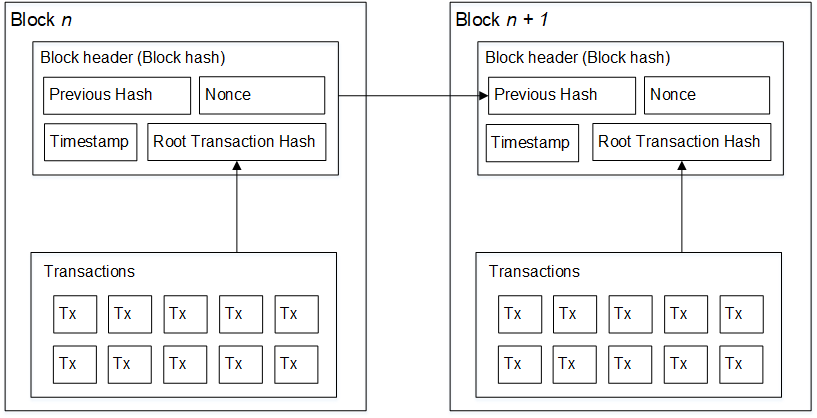
\includegraphics[width=.95\textwidth]{blocks-bitcoin}
    \caption{Composition of the Bitcoin blockchain. Work of a node consists of repeatedly hashing the block header, trying out different nonce every time.}
    \label{fig:blocks-bitcoin}
\end{figure}
% 
\subsubsection{Network of nodes}
Each node carries out work at its own pace, trying different values for nonce and hashing the block header. Essentially, this is simply trying using the brute force to produce a hash below a threshold. This process is also referred to as \textit{mining}. Once the hash is below the current threshold, a new block is mined. The new block is then broadcasted to all the nodes connected to the network~\cite{NakamotoBitcoin:System}. When a node receives a block it has not seen before, it first verifies the transactions in the block and then introduces it to its peers. The average time for a block to reach the whole network is 12.6 seconds~\cite{Decker2013InformationNetwork}. It is well below the block generation speed (1 block approximately every 10 minutes), however, it is not crucial for the network that every node has a copy of the latest block: ``\textit{If a node does not receive a block, it will request it when it receives the next block and realises it missed one.}''~\cite{NakamotoBitcoin:System}.
% 
\subsubsection{Transactions and accounts}
A Bitcoin transaction is the act of moving the funds from one account to another~\cite{Judmayer2017BlocksMechanisms}, as illustrated in Figure~\ref{fig:bitcoin-tx}. To explain this process, we must first define the notion of an account.

\begin{figure}[ht]
    \centering
    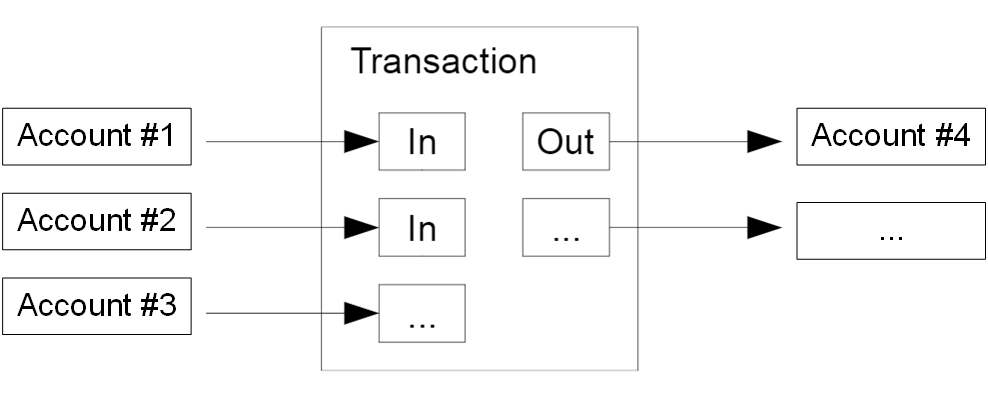
\includegraphics[width=\textwidth]{bitcoin-tx}
    \caption{A Bitcoin transaction representation. Each transaction has to have at least one input and one output. The inputs and outputs can have various values, but the total sum of the inputs needs to be equal to or greater than the number of outputs. The only exemption from this rule is the reward for the miner that found a new block. Such transaction only has outputs and no inputs. Taken from~\cite{NakamotoBitcoin:System}, edited.}
    \label{fig:bitcoin-tx}
\end{figure}

An account is a pair of a public and private key. Bitcoin uses the \acrfull{ecdsa} for the key pair generation~\cite{Decker2013InformationNetwork}. The account is identified by its public address, which is generated from the public key through a series of hashes. Figure~\ref{fig:public-address-gen} describes this process in further detail.
% 
\begin{figure}[p]
    \centering
    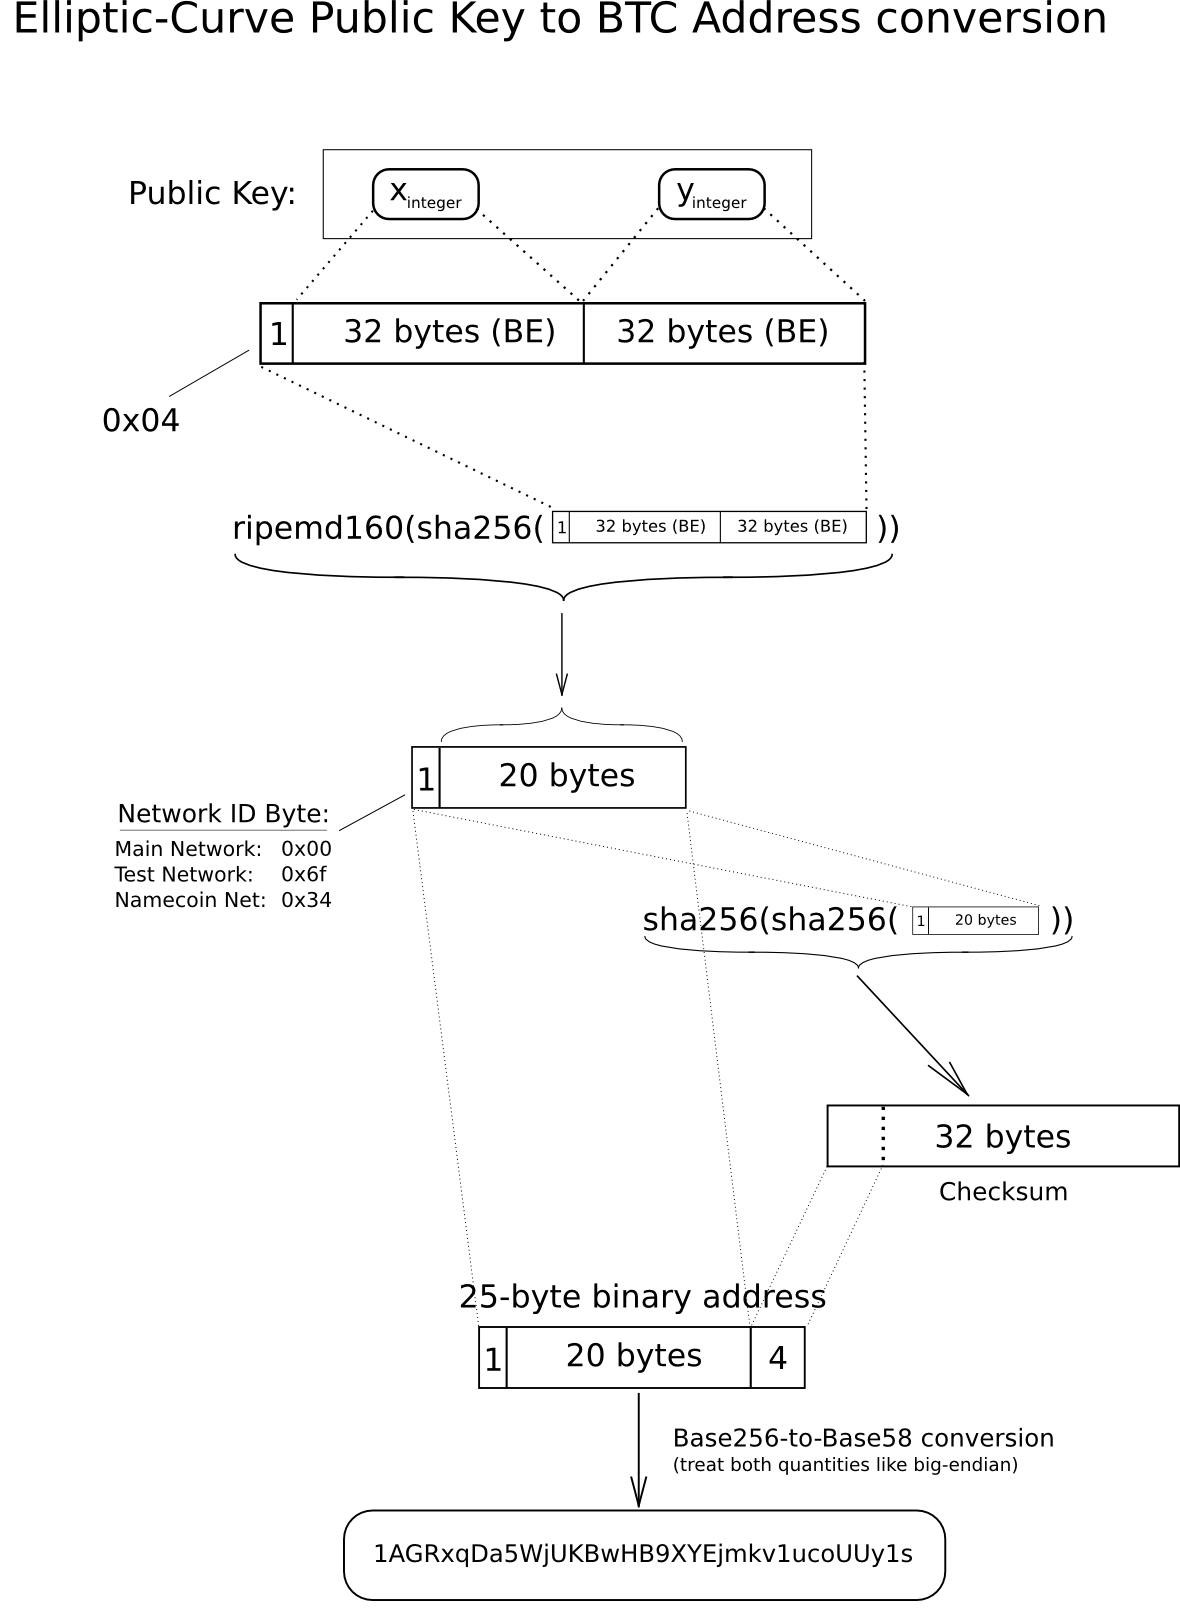
\includegraphics[height=.85\textheight]{PubKeyToAddr}
    \caption{First, a public key and a prefix are hashed using SHA-256 and then RIPEMD-160. This value is hashed twice with SHA-256 to generate a checksum. The result is composed of 1 network byte, RIPEMD-160 hash and first 4 bytes of checksum.}
    \label{fig:public-address-gen}
\end{figure}

A transaction contains a number of inputs and a number of outputs. The sum of inputs must be equal or greater than the sum of the outputs~\cite[p. 27]{Judmayer2017BlocksMechanisms}. In case the sum of the inputs of the transaction is greater than sum of the outputs, the excess is collected by the miner as the \textit{transaction fee}.

Every unit of the currency has a history of transactions up to its origin. This chain of ownership verifies the validity of that particular unit and serves as a proof, that the unit is not counterfeit. Transferring funds from one account to another comprises hashing the public address of the future owner and hash of the last transaction. The resulting hash is then singed with the private key of the previous owner~\cite{NakamotoBitcoin:System}, as illustrated in Figure~\ref{fig:chain-ownership}. Once the transaction is signed, it is distributed to the network and can be included in a block.
% 
\begin{figure}[ht]
    \centering
    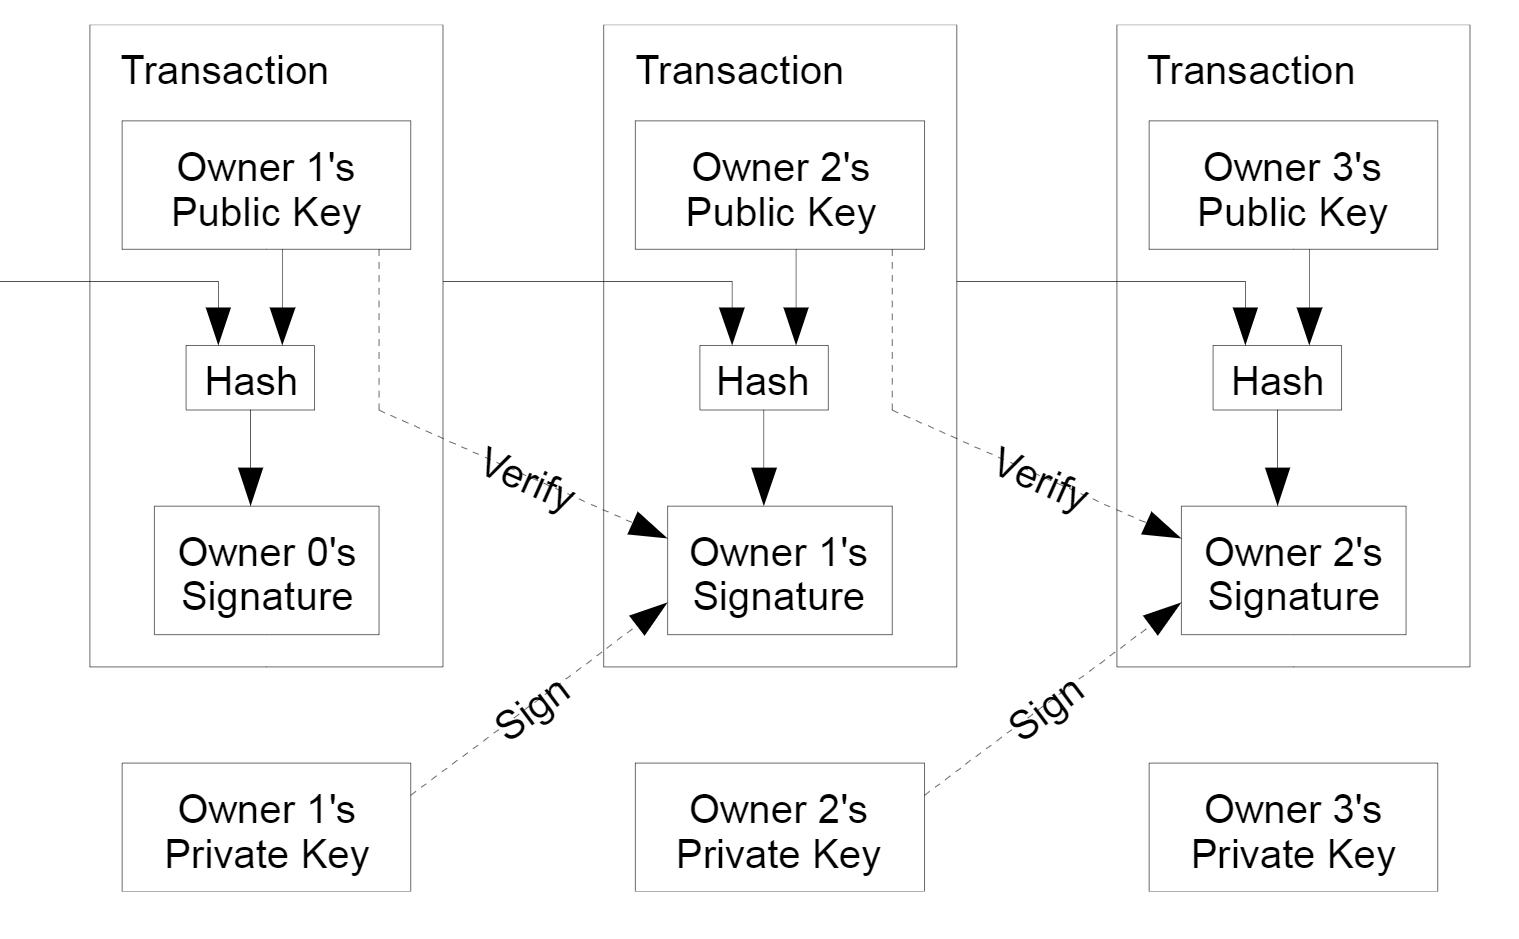
\includegraphics[width=.95\textwidth]{chain-ownership}
    \caption{Chain of ownership for unit of currency. Taken from~\cite{NakamotoBitcoin:System}.}
    \label{fig:chain-ownership}
\end{figure}

\subsubsection{Value}
Besides the system described above, the term `Bitcoin' also refers to a basic \textit{unit} of the currency. Bitcoin is further divisible into smaller units. The smallest unit is 1~Satoshi. 1~Bitcoin contains 100,000,000~Satoshi. 1~Bitcoin at the time of writing has a value of EUR~5~666. The value of Bitcoin is very volatile and has increased and decreased by tens or percents, sometimes even within hours~\cite{Adkisson2018WhyVolatile}. The peak in the value of Bitcoin has occurred on December~16,~2017 when 1 Bitcoin was traded for around USD~19,700~\cite{WolfieZhao2017BitcoinHigh}.

\subsubsection{Incentives}\label{sec:incentives}
A node that manages to successfully mine a block, collects fees from all the included transactions, which poses as an incentive for the nodes to stay honest and keep mining new blocks. In addition to the transaction fees, there is a reward associated with each newly mined block. This reward at the time of writing is 12.5 coins and halves every 210,000 blocks~\cite{Judmayer2017BlocksMechanisms}, with expected decrease again in 2020. The reward is a transaction with no inputs and is the only exception, where the outputs of a transactions are higher than its inputs. The reward for mining a block will decrease to zero approximately in 2140. The supply of the currency is therefore limited and there is an upper bound to the number of Bitcoins that will ever exist\footnotemark.

\footnotetext{As~\cite[p. 38]{Judmayer2017BlocksMechanisms} notes, this limit is only ensured pragmatically and is only valid if majority of the network observes this rule.}

\subsubsection{Altcoins}
The Bitcoin proposal and the first reference client were both published publicly. Not only this allowed for easy adoption within the community, it also enabled creation of cryptocurrencies derived from Bitcoin. These cryptocurrencies, that build on top of Bitcoin and only change few aspects of the system are known as \textit{altcoins}~\cite{Judmayer2017BlocksMechanisms}. Some of these currencies gained exchange value and are still in use by the general public. Others may be targeted on a specific use-case or are only used by narrow communities. Furthermore, some of these altcoins can also serve as proof-of-concept for any improvement proposals for the Bitcoin network~\cite{Tarasiewicz2015ChapterExperiments}. Litecoin, Dogecoin, Namecoin and Talkcoin\footnotemark are only few of the many examples of altcoins. Their differences from Bitcoin and their uses are shown in Table~\ref{tab:altcoins}.
% 
\footnotetext{\url{https://litecoin.org/}\\
\url{https://dogechain.info/}\\
\url{https://namecoin.org/}\\
\url{https://bitcointalk.org/index.php?topic=781207/} all accessed 18-05-2018}
% 
\begin{table}[ht]
    \centering
    \begin{tabularx}{\textwidth}{|l|X|m{10em}|}
         \hline
         \textbf{Name}&\textbf{Main difference from Bitcoin}&\textbf{Use}\\
         \hline
         \hline
         Litecoin&Shorter block time, different \acrshort{pow} algorithm&Value exchange\\
         \hline
         Dogecoin&Shorter block time&Humorous\\
         \hline
         Namecoin&Possible distributed data storage&Domain name registration (.bit), various other uses\\
         \hline
         Talkcoin&Possible message exchange between users, faster block time&Chatting\\
         \hline 
    \end{tabularx}
    \caption{Comparison of selected altcoins.}
    \label{tab:altcoins}
\end{table}

\subsubsection{Bitcoin (and other simple currencies)}
\subsubsection{Ethereum}

\subsection{Nomenclature}
Despite the existing definitions for words \textit{currency}, \textit{fiat currency} and \textit{cryptocurrency}, there are several naming convention in use today. This paragraph describes, which terms will be used further in this report.

The value of many cryptocurrencies is not backed by any commodity and it depends entirely on the supply/demand relationship. Therefore, by the definition, these cryptocurrencies are also fiat currencies. However, in the literature, the term \emph{fiat currency} is often used when referring to traditional, government issued currencies only. For the rest of this paper we will therefore keep this naming. Regular currencies, such as dollars, euros or crowns will be referred to as fiat currencies.

Virtual, digital money such as Bitcoins, Ether, Litecoin and similar are in some sources named 'coin currencies'. However, in this paper they will be referred to as 'cryptocurrencies' instead, as this is the most common term.